\begin{figure}[t]
\vspace*{-5ex}
\centering
\hspace*{1.8em}
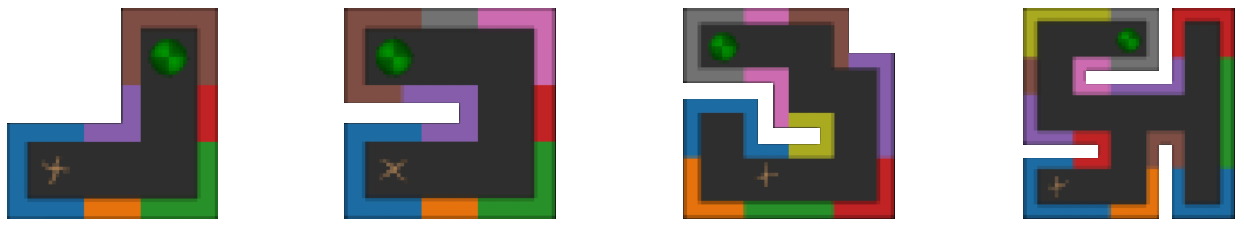
\includegraphics[width=0.93\textwidth]{mazes/tasks} \\[2ex]
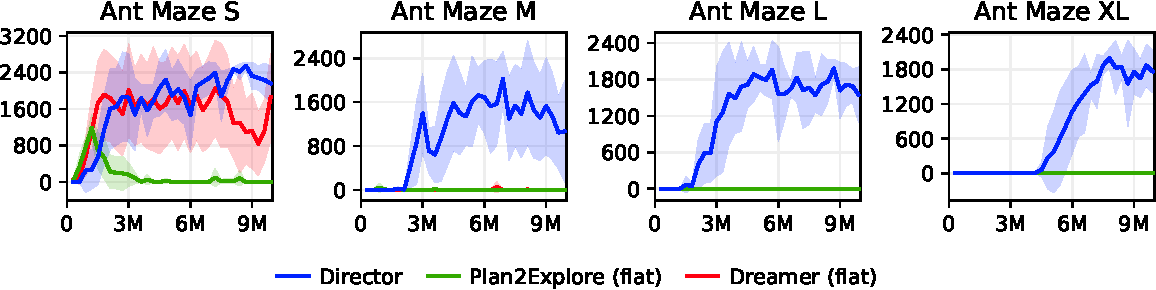
\includegraphics[width=\textwidth]{mazes/curves}
\caption{Egocentric Ant Maze benchmark. A quadruped robot is controlled through joint torques to navigate to a fixed location in a 3D maze, given only first-person camera and proprioceptive inputs. This is in contrast to prior benchmarks where the agents received their global XY coordinate or top-down view. The only reward is given at time steps where the agent touches the reward object. Plan2Explore fails in the small maze because the robot flips over too much, a common limitation of low-level exploration methods. Director solves all four tasks by breaking them down into manageable subgoals that the worker can reach, while learning in the end-to-end reinforcement learning setting.}
\label{fig:mazes}
\end{figure}
